\subsection[conic sections]{Conic Sections}

\textit{Translate between the \textbf{geometric description} and \textbf{the equation} for a conic section}

\vspace{1cm}

\begin{center}
    \begin{tabular}{|l|l|p{3.5cm}|}
        \hline
        section & equation & geometric description \\ \hline
        circle  & $x^2 + y^2 = a^2$ & the set of all point in a plane equidistant from a center point.\\ \hline
        parabola  & $y^2 = 4ax$ & the locus of points in that plane that are equidistant from the directrix and the focus.\\ \hline
        ellipse  & $\frac{x^2}{a^2} + \frac{y^2}{b^2} = 1$ & for all points on the curve, the sum of the two distances to the focal points is a constant.\\ \hline
        hyperbola & $\frac{x^2}{a^2} - \frac{y^2}{b^2} = 1$ & for all points on the curve, the difference of the two distances to the focal points is a constant.\\ \hline
        
    \end{tabular}
\end{center}



\subsubsection[cones]{Cones}

\begin{figure}[h!]
    \begin{center}
        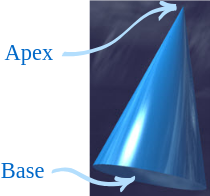
\includegraphics[scale=.45]{./public/images/cone-parts}
        \caption{a cone has an apex and a base}
    \end{center}
\end{figure}

\begin{enumerate}
    \item a cone has a circle at one end and a point at the other
    \item a cone can be made by rotating a triangle
    \item surface area
    $$SA_{cone} = \pi r(s + r)$$
    $$s = \sqrt{h^2 + r^2}$$
\end{enumerate}

\begin{figure}[h!]
    \begin{center}
        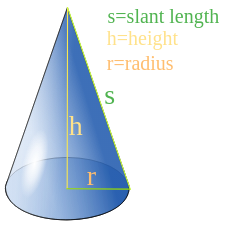
\includegraphics[scale=.45]{./public/images/cone-surface-area}
    \end{center}
\end{figure}


\subsubsection[conics]{Conic Sections}

\paragraph*{eccentricity}

The ratio of the distances from a curve to a focus and a curve to a directrix is called the \textbf{eccentricity}.

\paragraph*{latus rectum}

The Latus Rectum is a line passing through the foci of a conic section and parallel to the directrix. I

\subsubsection[ellipse]{Ellipse}

the set of all points (x,y) in a plane the \textbf{sum} of whose distances from two distinct points(the foci) is constant.

\paragraph*{eccentricity}

$$ 0 < eccentricity < 1 $$

$$ \frac{x^2}{a^2} + \frac{y^2}{b^2} = 1$$


\begin{figure}[h!]
    \begin{center}
        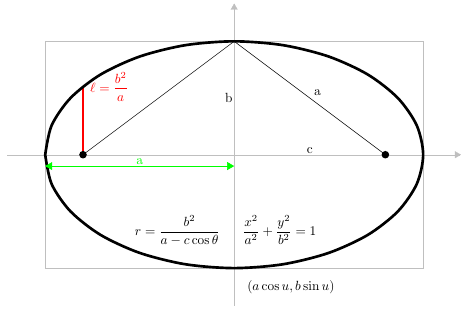
\includegraphics[scale=.45]{./public/images/ellipse2}
    \end{center}
\end{figure}

\paragraph*{circle}

The circle is a special case of an ellipse. if $eccentricity = 0$, the ellipse is a circle.

\subsubsection[hyperbola]{Hyperbola}

hyperbola - the set of all points (x,y) in a plane the \textbf{difference} of whose distances from two distinct points is constant
$$ \frac{x^2}{a^2} - \frac{y^2}{b^2} = 1$$

\begin{figure}[h!]
    \begin{center}
        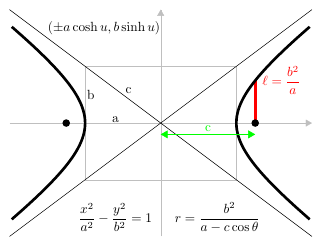
\includegraphics[scale=.45]{./public/images/hyperbola2}
    \end{center}
\end{figure}